\chapter*{22.07. --- Komu w drogę, temu czas}

\section*{Ostatnie sprawunki}

\indent Przed wyruszeniem we właściwą trasę musieliśmy jeszcze załatwić kilka sprawunków w Keflavíku. Mam tu na myśli wszelkie rzeczy, których z różnych względów ,,formalno-prawnych'' po prostu nie dało się załatwić w Polsce.
Najpierw zawitaliśmy na stację benzynową Olís \footnote{\href{https://www.google.com/url?q=https\%3A\%2F\%2Fmaps.google.com\%2Fmaps\%3Fq\%3D63.979816\%2C-22.54672}{mapa z zaznaczoną stacją benzynową}}, by zakupić naboje do palników gazowych.

W sumie nie było takiej konieczności --- równie dobrze mogliśmy skorzystać z darmowych butli, które turyści już odlatujący z wyspy masowo porzucają na kempingach położonych w promieniu ok. 50 km od stołecznego lotniska. Podobno na kempingu w Garður --- tuż obok lotniska --- leżą całe hałdy tych naboi i to np. w 2/3 pełne.
Następnie zahaczyliśmy o warsztat wulkanizacyjny \footnote{\href{https://www.google.com/url?q=https\%3A\%2F\%2Fmaps.google.com\%2Fmaps\%3Fq\%3D63.982619\%2C-22.546328}{mapa z zaznaczonym zakładem wulkanizacyjnym}}, gdzie sprawnie dobiliśmy\footnote{in. dopompowaliśmy} opony do ponad 4 atmosfer.

\hint{Naboje gazowe można próbować ,,upolować'' na kempingach znajdujących się w pobliżu lotniska (czyli w promieniu około 50 km, np. w Garður albo w Grindavíku). Zdarzają się nawet naboje w 2/3 pełne!}

\hint{Do jazdy po asfalcie lepiej mieć opony naprawdę twarde, czyli napompowane do maksymalnego dopuszczalnego ciśnienia, gdyż dzięki temu znacznie zmniejszają się opory toczenia. Mówiąc po ludzku --- zajedziesz dalej, szybciej, mniej się męcząc :)}

Kolejnym punktem programu był supermarket sieci Bonus --- bodaj najtańszej na Islandii. Nie będę się tu rozpisywał za bardzo o tym, w jaki zachwyt wprawiły nas ceny produktów i ich wybór, gdyż \href{http://www.roboppy.net/food/2009/04/iceland-day-1-part-ii-reykjavik-bonus-supermarket-skyr.html}{to zrobili już inni przed nami}. Wspomnę tylko o jednym naszym odkryciu --- chodzi o przecier ananasowy marki EuroShopper. Trzypak puszek, każda po 227 g (z czego 70\% to ananas, a reszta --- sok ananasowy, a nie syrop) kosztował\textellipsis 40 kr! Czyli 60 kr --- jakieś 1,50 zł --- za kilogram. Aż żal nie kupić! Te ananasy doskonale pełniły rolę deseru --- oczywiście gdy tylko Bonus był pod ręką\textellipsis

\img{./photos/x-s-2014-07-22_14-53-31__2.jpg}{keflavik_metal_guys}{Fantazja Islandczyków --- uliczni tancerze\textellipsis}

%\begin{figure}[h]
%\centering
%\begin{subfigure}{.5\textwidth}
%  \centering
%  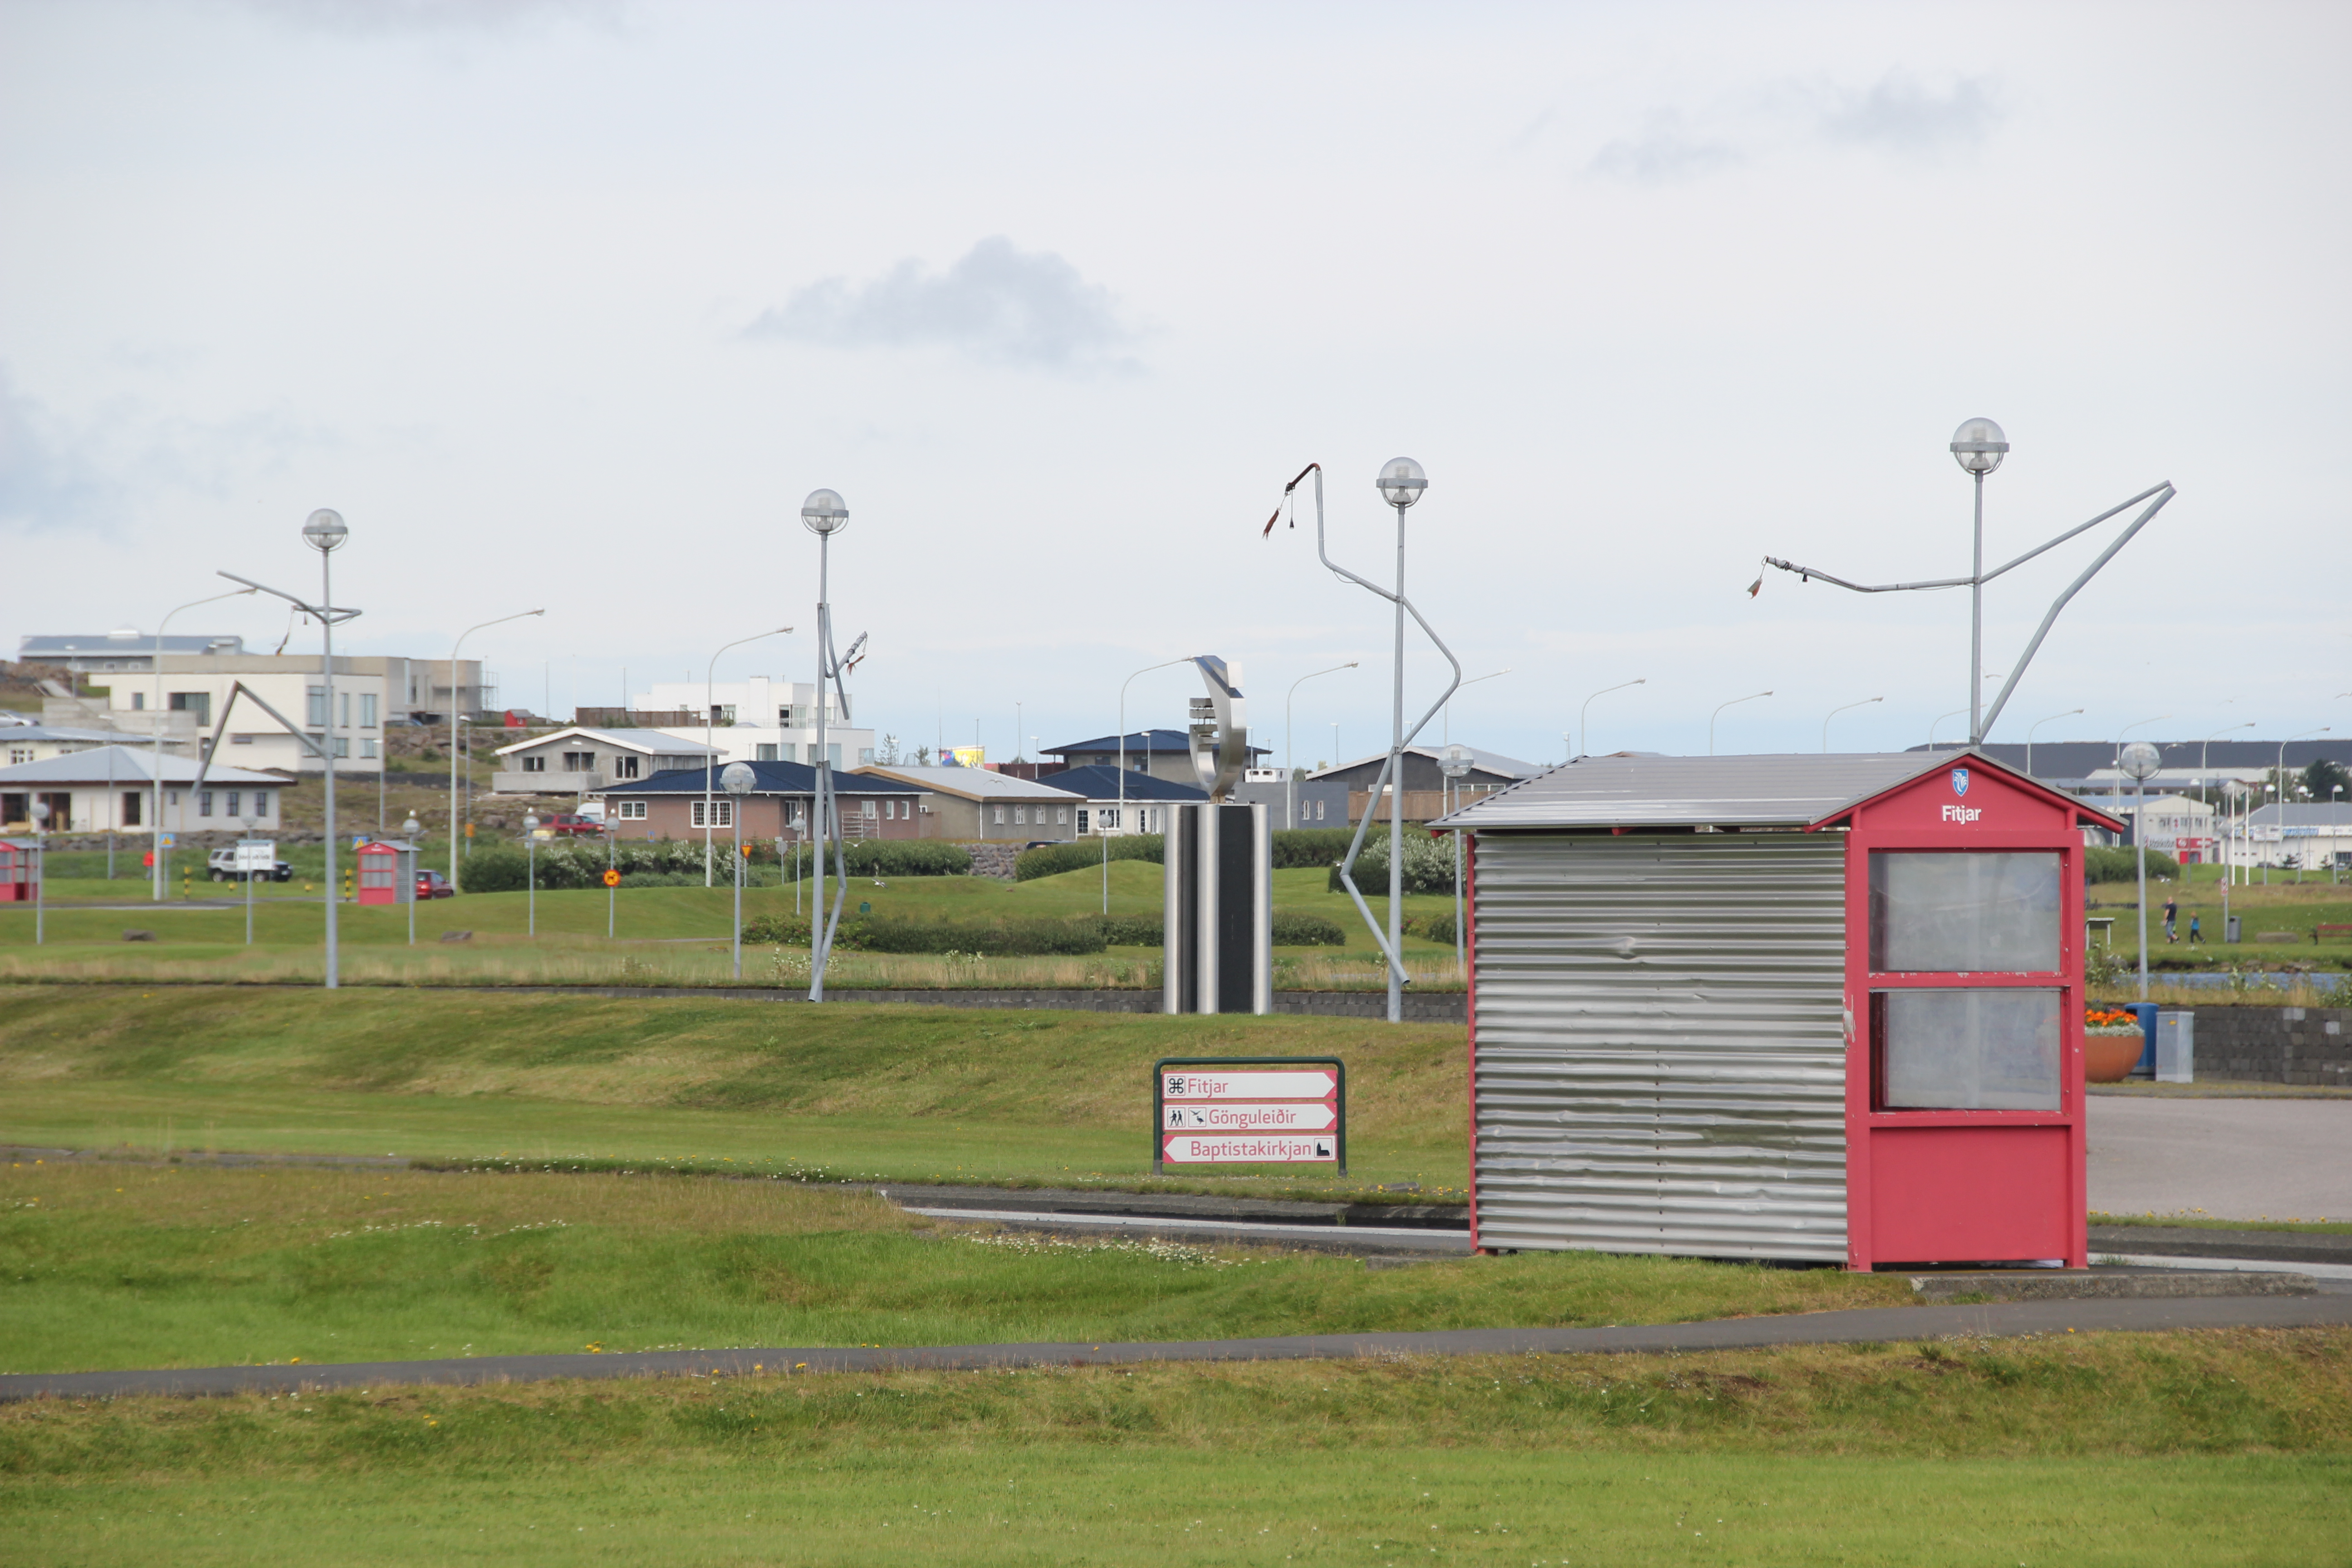
\includegraphics[width=.9\textwidth]{./photos/2014-07-22_14-53-31__2.jpg}
%  \caption{A subfigure}
%  \label{fig:keflavik_metal_guys}
%\end{subfigure}%
%\begin{subfigure}{.5\textwidth}
%  \centering
%  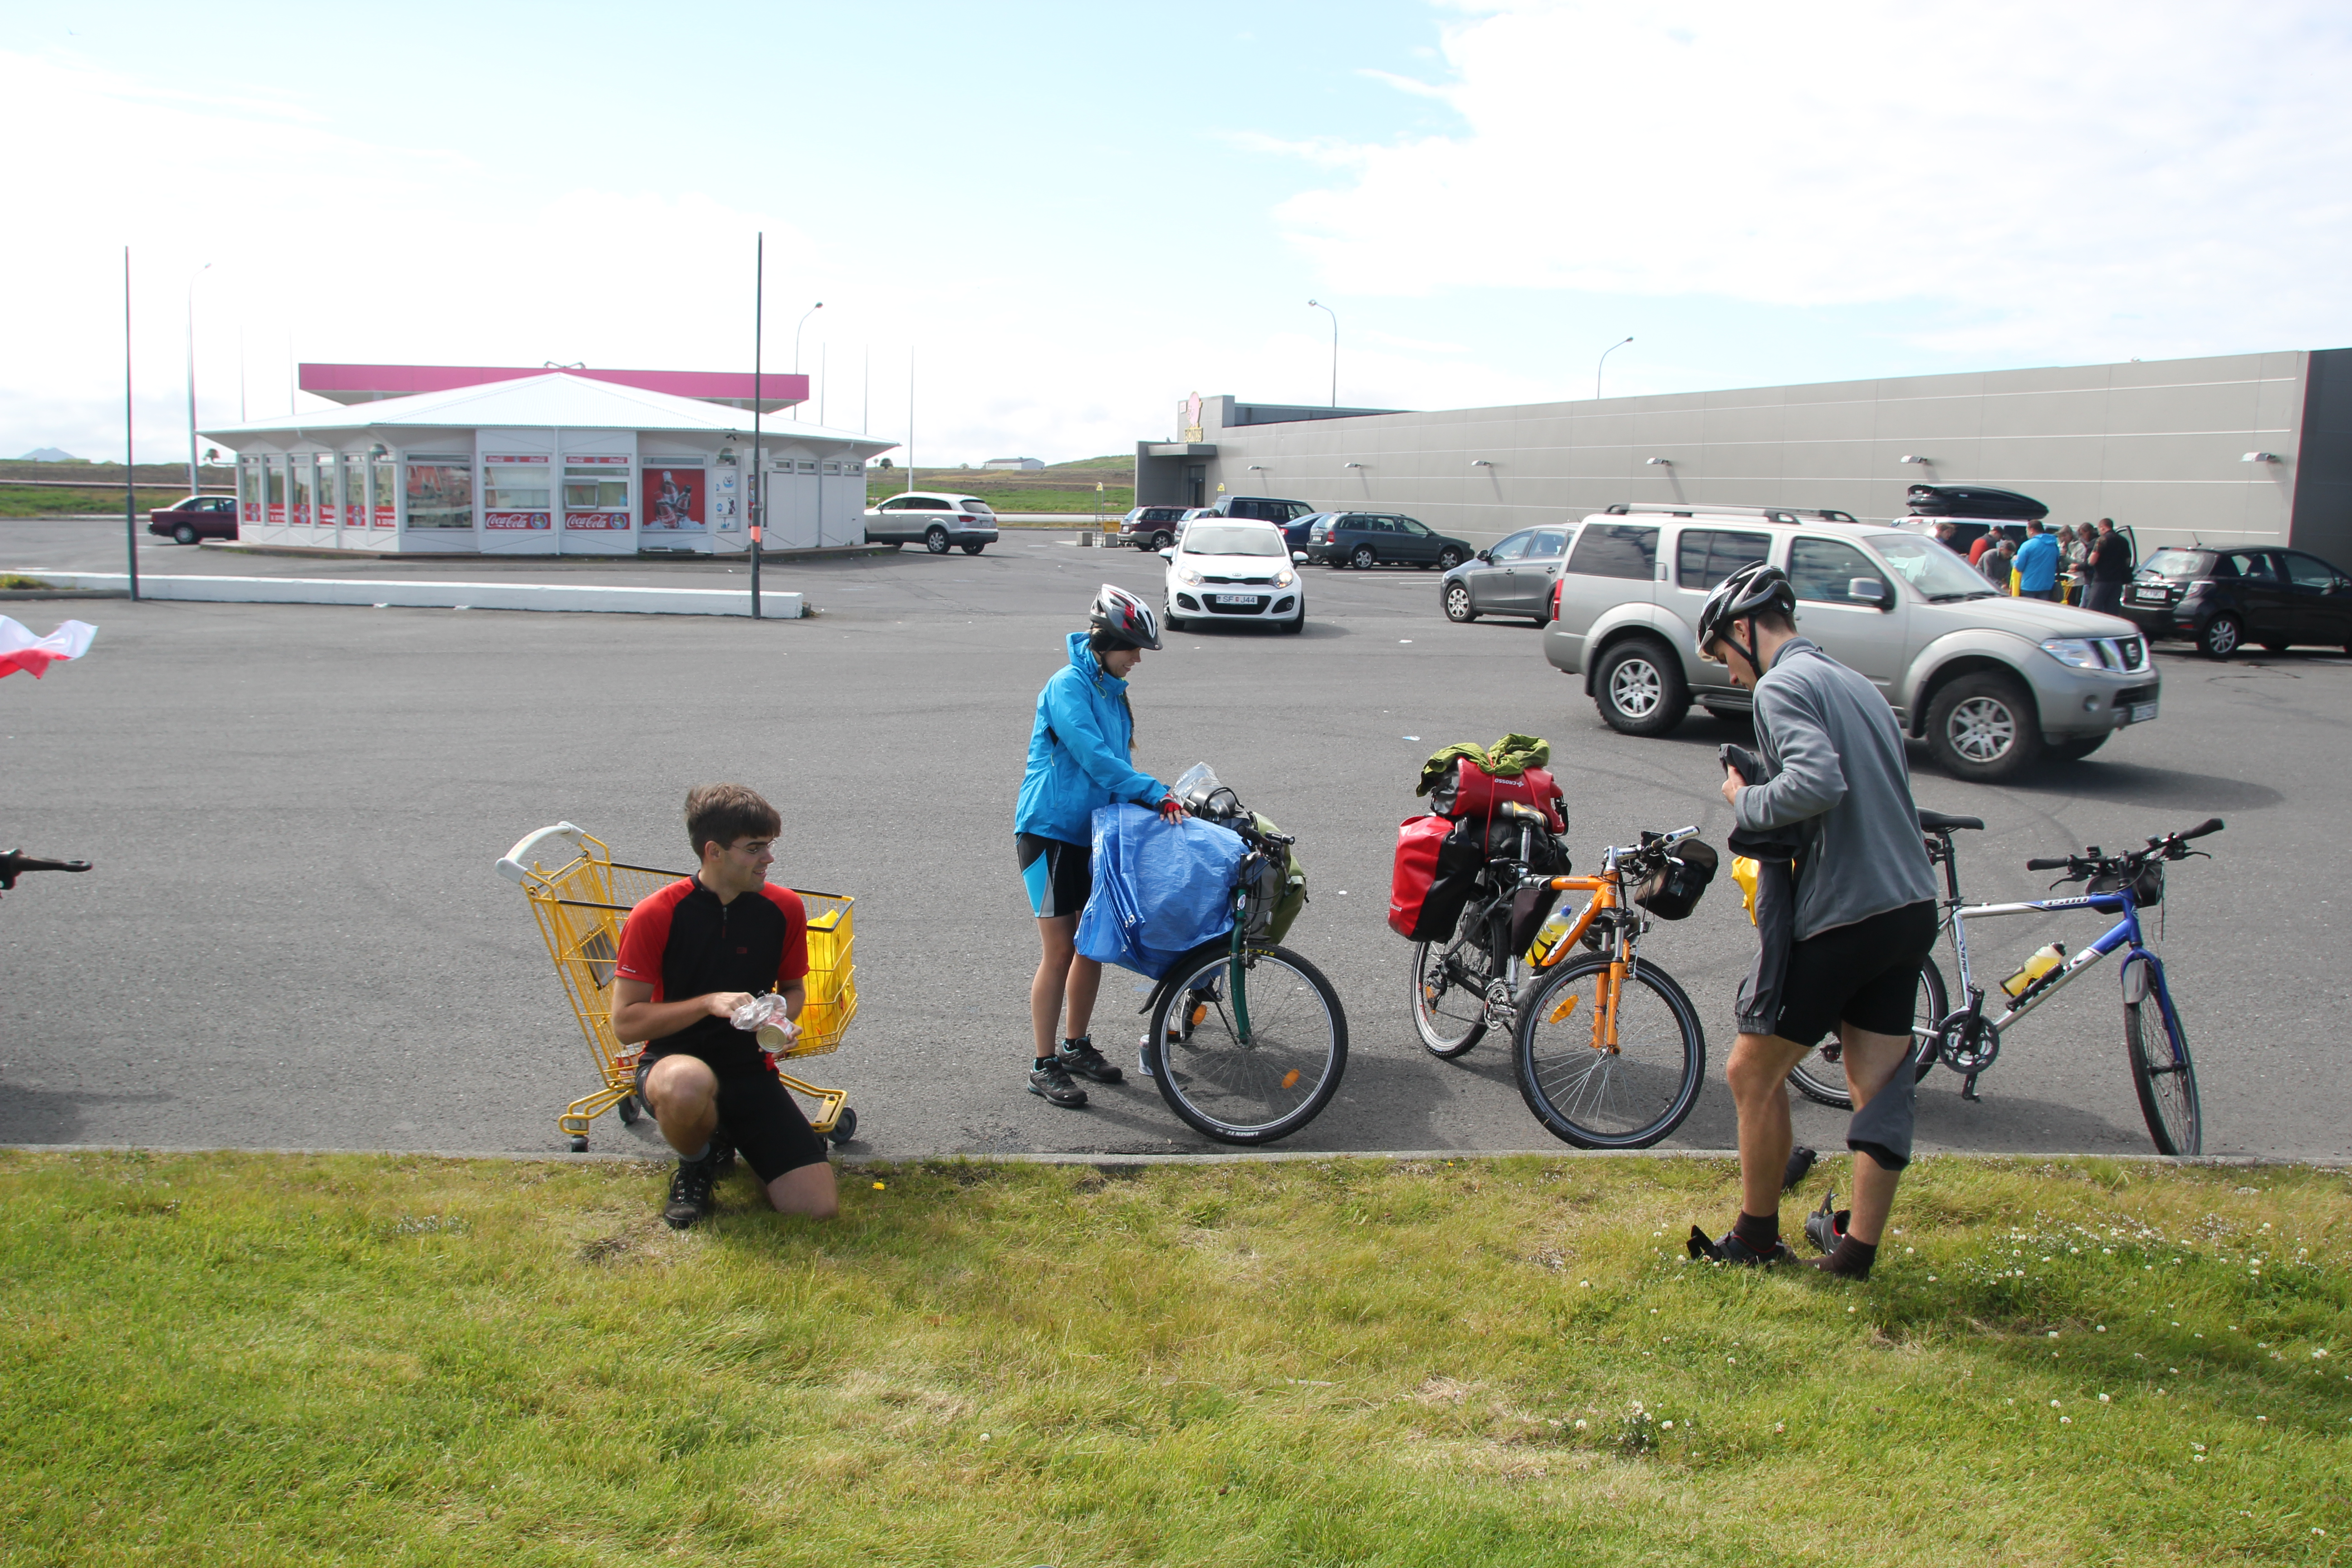
\includegraphics[width=.9\textwidth]{./photos/2014-07-22_14-54-31__3.jpg}
%  \caption{A subfigure}
%  \label{fig:keflavik_breakfast}
%\end{subfigure}
%\end{figure}

Posileni, pełni sił, ruszyliśmy do centrum Keflavíku, do oddziału Landsbanki \footnote{\href{https://www.google.com/url?q=https\%3A\%2F\%2Fmaps.google.com\%2Fmaps\%3Fq\%3D63.995522\%2C-22.548067}{mapa z zaznaczonym oddziałem Landsbanki}} --- takiego tutejszego PKO\footnote{Powszechna Kasa Oszczędności przez wiele lat stanowiła główny komercyjny bank Polski.} --- by wymienić trochę waluty. Niby na lotnisku był bankomat, ale niektóre karty średnio z nim współpracowały, a do tego dziewczyny chciały wymienić trochę euro w~gotówce na korony\textellipsis

\hint{Na Islandii naprawdę wszędzie można płacić kartą. Nawet na kempingach w środku interioru! Jedyne, co warto mieć ze sobą, to żelazną rezerwę monet o nominale 100 kr --- na wielu kempingach zainstalowane są ,,dozowniki ciepłej wody'', które przyjmują pięć takich monet i w zamian umożliwiają wzięcie 5-minutowego ciepłego prysznica. Czasem da się rozmienić banknoty na monety na kempingu, lecz w myśl zasady ,,przezorny zawsze ubezpieczony'' znacznie lepiej zrobić to zawczasu w jakimś sklepie czy na stacji benzynowej.}

Ostatnim puntem był zakup czegoś, co umożliwi nam dzwonienie z islandzkiego numeru komórkowego oraz korzystanie z internetu --- wybór padł na Vodafone (biuro tej firmy mieściło się koło polskiego marketu), który oferował 3 GB danych za około 50 zł. O ile z zakupem prepaidu nie mieliśmy problemu, o tyle aktywacja internetu wymagała już znacznie więcej zachodu. Nie dość, że operacja odbywała się poprzez infolinię Vodafone, to jeszcze niezbędne było posiadanie karty kredytowej --- szczęśliwie mieliśmy w odwodzie w Polsce posiadacza takowej. Chcę przy tym podkreślić, że internet miał nam służyć nie tylko do zabawy facebookiem, ale o tym później\textellipsis

\hint{Zawczasu, przed wyjazdem z Polski, zorientuj się kto z rodziny, przyjaciół lub znajomych posiada kartę kredytową i będzie skłonny podać ci jej numer, datę ważności oraz kod CVV. Dodatkowo zapisz imię i nazwisko posiadacza karty w takim brzmieniu, jak na karcie (czyli z uwzględnieniem polskich liter lub ich braku). Istnieje pewna grupa usług --- np. aktywacja pakietu internetowego, zakup niektórych biletów online --- których nie da się załatwić przy użyciu zwykłej karty debetowej!}

Keflavík opuściliśmy ostatecznie o 15:00, przy (wciąż jeszcze) słonecznej pogodzie.

\hint{Islandia to olbrzymi obszar i ciężko zawczasu dowiedzieć się o każdej atrakcji i o każdym interesującym miejscu na trasie. Warto więc korzystać intensywnie z informacji turystycznych, zbierać (i przeglądać!) foldery reklamowe oraz pytać innych turystów (najlepiej też rowerzystów, bo ci będą w stanie np. przestrzec cię przed trudnościami terenowymi). W Keflavíku znajduje się Centrum Informacji Turystycznej --- lokalizację znajdziesz na ich profilu na Google+ (\url{https://plus.google.com/111960041675886065623/about?gl=pl\&hl=en}).}

\section*{Pierwsze godziny w trasie}

Pierwsze kilometry i już mocne zderzenie z islandzką naturą --- jedziemy przez pustkowia. Po lewej, po prawej, jak okiem sięgnąć lawa i niewielkie skałki. Nic dziwnego, że obszar ten --- jako jeden z trzech na Islandii --- służył NASA do prowadzenia treningów dla astronautów przed misją Apollo.

Kawałek przed Hafnir przyplątał się do naszej grupy pies, którego ochrzcziliśmy imieniem Posejdon (od \href{https://www.facebook.com/120832791270880/photos/a.612815058739315.1073741825.120832791270880/612815132072641/?type=3&theater}{pomnika planety Neptun}, który stał w miejscu zdarzenia). Pies ten biegł za nami aż do \href{http://www.visitreykjanes.is/searchresults/attraction/bridge-between-continents}{Kładki Między Kontynentami}. Nie byłoby w tym nic aż tak specjalnego gdyby nie to, że nasz nowy towarzysz urzekł nas swym polowaniem na samochody: gdy zauważył nadjeżdżający pojazd, zaczajał się na poboczu i potem w ostatniej chwili wypadał na jezdnię --- tuż przed maskę --- głośno ujadając. Albo niesamowicie odważny albo niesamowicie głupi ;-)

Już daje się nam we znaki wiatr oraz liczne (na szczęście krótkie) stromsze podjazdy. Walka z takim kombo jest szczególnie ciężka dla tych osób, które nie jeździły ostatnio za wiele.

\img{./photos/x-s-2014-07-22_18-05-39__5.jpg}{first_hours_on_iceland}{Pustkowia półwyspu Reykjanes}

\img{./photos/x-s-2014-07-22_18-25-14__8.jpg}{neptune_monument}{Pomnik planety Neptun}

\clearpage


\hint{Podczas jazdy na rowerze pracują nieco inne mięśnie niż np. podczas wycieczek górskich. Bieganie, pływanie, orbitrek --- wszystko to oczywiście zwiększa wydolność organizmu, lecz nic nie zastąpi odpowiedniej liczby przejechanych kilometrów! :)}

Słońce było tylko na zachętę --- szybko schowało się za chmury i zrobiła się typowa islandzka aura --- z mniej lub bardziej intensywnymi opadami deszczu\textellipsis A trzeba wiedzieć, że tu nie ma się gdzie schować --- żadnych przydrożnych sklepów, barów, nawet wiat PKS-u! Tak więc, siłą rzeczy, mimo deszczu jedziemy dalej. Zresztą\textellipsis nie lało tylko kropiło, czyli nawet nie byłoby sensu przeczekiwać takiego opadu. Klimat tu bowiem taki, że można by się nie doczekać momentu ,,wypadania''.

\section*{Grindavík}

Gdy byliśmy już na obrzeżach Grindavíku powstał problem --- szukać miejsca na nocleg już teraz, czy może jechać jeszcze kawałek dalej? Cała ekipa była dość jednomyślna: \emph{Nie, nie jedziemy już dalej --- jest za późno (była 19:00 --- red.) no i warto byłoby się nie zarżnąć od razu pierwszego dnia. Lepiej wyruszyć wcześniej nazajutrz, ale przynajmniej dziś odespać podróż!} Tu konieczne jest słowo komentarza --- berlińczycy\footnote{Ci, którzy lecieli na Islandię z Berlina: Put, Kasia i Karolina.} nie spali ani w Polskim Busie, ani koczując na lotnisku Schönefeld, ani też w samolocie. Zatem byli non-stop na chodzie przez 30 godzin, a ze względu na późny przylot i długie czekanie na bagaż noc w Ásbrú też była zarwana\textellipsis Tak więc po przejechaniu 50 km rozbiliśmy się na kempingu w Grindavíku.

Kemping można zaliczyć do klasy ,,all inclusive'', bo posiada ,,świetlicę'' (ogrzewanie podłogowe!) z w pełni wyposażonym aneksem kuchennym (sztućce, garnki, płyty indukcyjne, toster\textellipsis), a prysznice są w cenie. W kuchni całą jedną szafkę zajmował ,,free stuff'' --- nie tylko rzeczy spożywcze, ale też gospodarcze (np. są wspomniane naboje gazowe).

\img{./photos/x-s-2014-07-23_11-11-19__6.jpg}{grindavik_cantine}{Jadalnia kempingu w Grindavíku}

\hint{Będąc w kuchni na kempingu warto przeglądnąć cały asortyment opatrzony napisem ,,free food'' i ,,free stuff'', gdyż często można tam natrafić na towary luksusowe --- porządną herbatę, konserwy, słodycze, płatki śniadaniowe\textellipsis Należy jednak zwracać uwagę na termin przydatności do spożycia oraz organoleptycznie zbadać faktyczny stan produktu (np. otwartego mleka lepiej nie tykać ;-)}

Na obiadokolację z radością pochłaniamy spaghetti z mięsem ze słoika (polskie, domowe, zawekowane mięso --- mniam!), sosem i warzywami z puszki. Przekąszamy ciasteczkami i niezwłocznie udajemy się na spoczynek --- większość z nas nawet bez mycia się, bo tak bardzo jesteśmy ,,wcięci''\textellipsis

\hint{Kupując warzywa i sosy w puszcze zwróć uwagę na ,,gęstość'' produktu, tj. stosunek wagi netto (po odcieku) do wagi brutto --- bo po co wozić ze sobą puszkowaną wodę?! Na Islandii bezkonkurencyjna pod tym względem okazała się mieszanka warzyw Euroshopper, w której wspomniany współczynnik wynosił\linebreak około 0,95.}

Ponieważ mamy internet i założone wydarzenie na fb (co by nie musieć powtarzać po parę razy tego samego --- gdzie jesteśmy i co robimy --- a to rodzinie, a to wszystkim znajomym), więc co jakiś czas Put informuje nas \emph{,,O! Mamy 5 lajków i 3 komentarze!''}. Hm\textellipsis może należało założyć profil fb? Wtedy moglibyśmy jeszcze korzystać ze statystyk\textellipsis

W ogóle (w miarę) swobodny dostęp do internet wprowadza też nową jakość wieczorami, przed spaniem. W pewnym momencie rozlega się dramatyczne wołanie \emph{,,Pucie, zrobisz modem?''}, a chwilę później \emph{,,Pucie, przełożysz komórkę bliżej naszego namiotu? Bo coś słaby zasięg\textellipsis''}

\vspace{16pt}

Aha, a na zakończenie --- cytat dnia:
\epigraph{,,Czuję się, jakbym była na Islandii od tygodnia\textellipsis''}{--- \textup{Karolina}}

